
\documentclass{article} % For LaTeX2e
\usepackage{icais2025_conference,times}

% Optional math commands from https://github.com/goodfeli/dlbook_notation.
\input{math_commands.tex}

\usepackage{hyperref}
\usepackage{url}
\usepackage{graphicx}
\usepackage{subfigure}
\usepackage{booktabs}

% For theorems and such
\usepackage{amsmath}
\usepackage{amssymb}
\usepackage{mathtools}
\usepackage{amsthm}

% Custom
\usepackage{multirow}
\usepackage{color}
\usepackage{colortbl}
\usepackage[capitalize,noabbrev]{cleveref}
\usepackage{xspace}
\usepackage{hyperref}
\hypersetup{
    colorlinks=true,
    linkcolor=blue!70!black,
    citecolor=green!60!black,
    urlcolor=red!60!black
}
\usepackage{url}


\title{Train for the Worst, Plan for the Best: Enhancing Token Ordering in Masked Diffusions}

% Authors must not appear in the submitted version. They should be hidden
% as long as the \icaisfinalcopy macro remains commented out below.
% Non-anonymous submissions will be rejected without review.

\author{Antiquus S.~Hippocampus, Natalia Cerebro \& Amelie P. Amygdale \thanks{ Use footnote for providing further information
about author (webpage, alternative address)---\emph{not} for acknowledging
funding agencies.  Funding acknowledgements go at the end of the paper.} \\
Department of Computer Science\\
Cranberry-Lemon University\\
Pittsburgh, PA 15213, USA \\
\texttt{\{hippo,brain,jen\}@cs.cranberry-lemon.edu} \\
\And
Ji Q. Ren \& Yevgeny LeNet \\
Department of Computational Neuroscience \\
University of the Witwatersrand \\
Joburg, South Africa \\
\texttt{\{robot,net\}@wits.ac.za} \\
\AND
Coauthor \\
Affiliation \\
Address \\
\texttt{email}
}

% The \author macro works with any number of authors. There are two commands
% used to separate the names and addresses of multiple authors: \And and \AND.
%
% Using \And between authors leaves it to \LaTeX{} to determine where to break
% the lines. Using \AND forces a linebreak at that point. So, if \LaTeX{}
% puts 3 of 4 authors names on the first line, and the last on the second
% line, try using \AND instead of \And before the third author name.

\newcommand{\fix}{\marginpar{FIX}}
\newcommand{\new}{\marginpar{NEW}}

%\iclrfinalcopy % Uncomment for camera-ready version, but NOT for submission.
\begin{document}


\maketitle

\begin{abstract}
Masked diffusion models (MDMs) have emerged as a powerful paradigm for generative modeling over discrete domains. However, their training often involves solving computationally intractable problems, while their inference capabilities remain underutilized. In this work, we propose to enhance the performance of MDMs by introducing adaptive inference strategies that allow for dynamic token ordering during decoding. We demonstrate that by sidestepping computationally heavy subproblems, pretrained MDMs can achieve significant performance improvements on complex tasks such as logic puzzles. Our experiments show that adaptive inference boosts Sudoku solving accuracy from less than 7\% to approximately 90\%, even outperforming autoregressive models with significantly more parameters. This work opens new avenues for leveraging the strengths of MDMs in discrete generative tasks.
\end{abstract}

\section{Introduction}
Masked diffusion models (MDMs) have gained traction for their ability to model complex data distributions in discrete spaces, yet they face significant challenges during training and inference. In particular, the computational complexity of their training processes and the limitations of fixed decoding strategies can hinder their usability in practical applications. Existing literature emphasizes the efficacy of autoregressive models (ARMs) for structured tasks, yet fails to explore adaptive inference strategies that exploit the flexibility of MDMs during inference. This paper addresses this gap by proposing adaptive token ordering strategies, which enhance MDMs' performance on complex generative tasks, particularly in solving logic puzzles. Our findings reveal that adaptive inference significantly improves accuracy and opens pathways for further research in generative modeling.

\begin{figure}[h!]
\centering
\subfigure[Baseline Loss Curves Over Epochs]{
    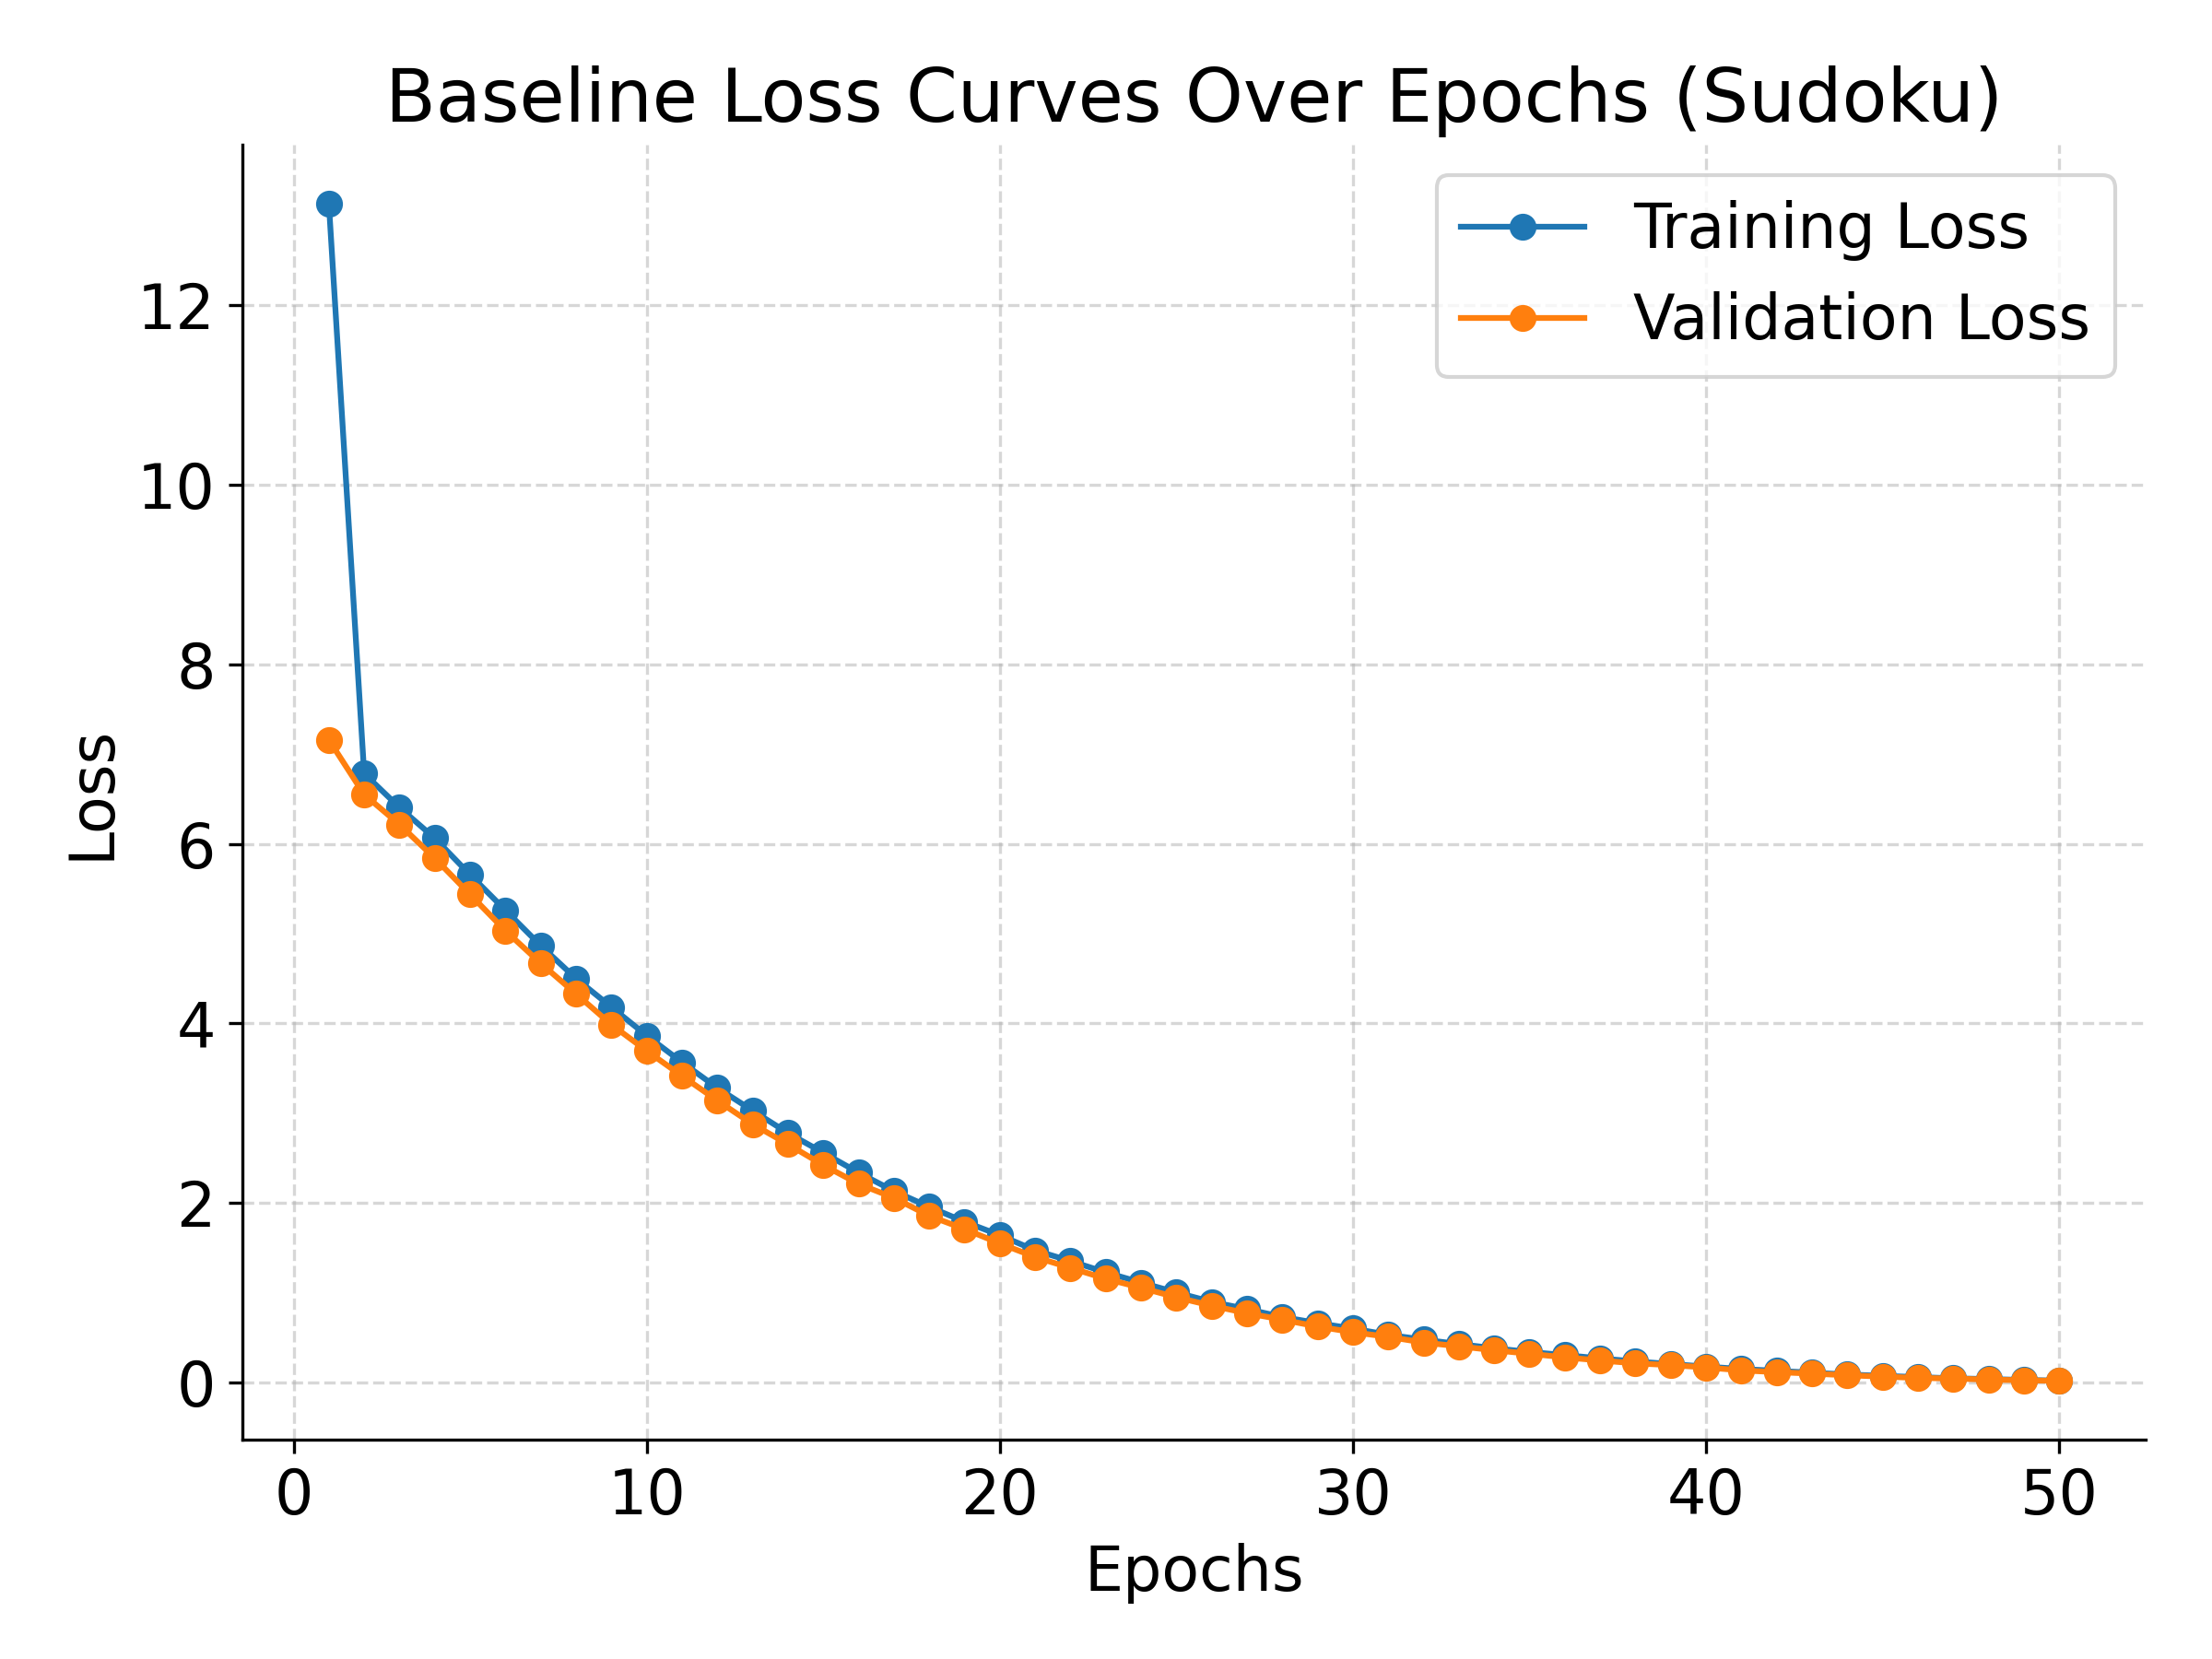
\includegraphics[width=0.50\textwidth]{img/1_baseline_loss_curves.png}
    \label{fig:1_baseline_loss_curves}
}
\subfigure[Activation Function Ablation]{
    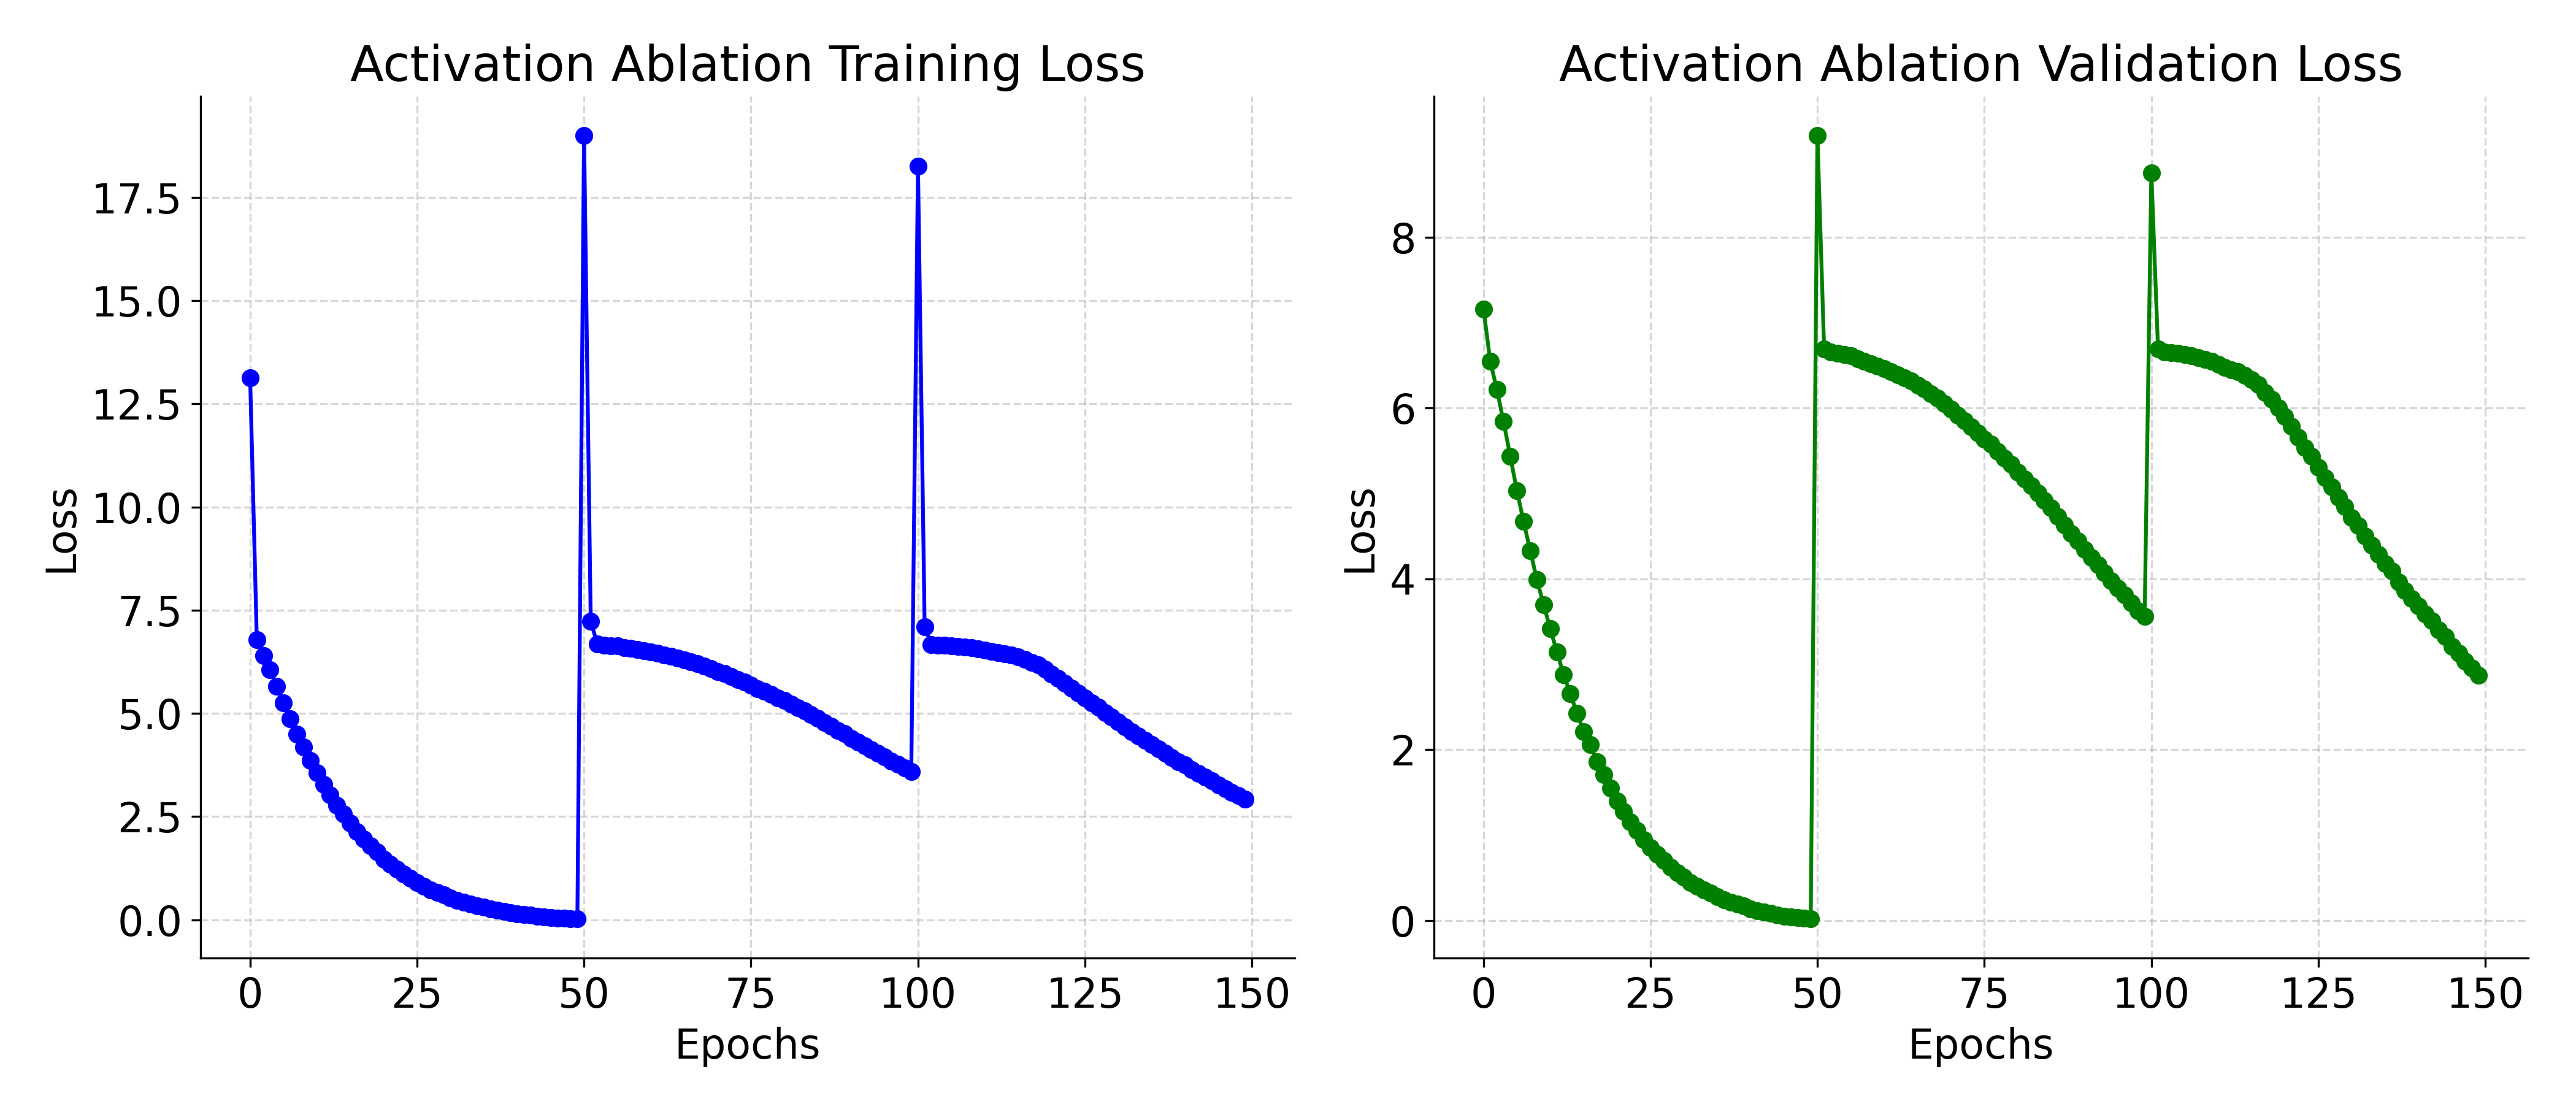
\includegraphics[width=0.70\textwidth]{img/2_activation_functions_loss.png}
    \label{fig:2_activation_functions_loss}
}
\subfigure[Dataset Variation Loss Curves]{
    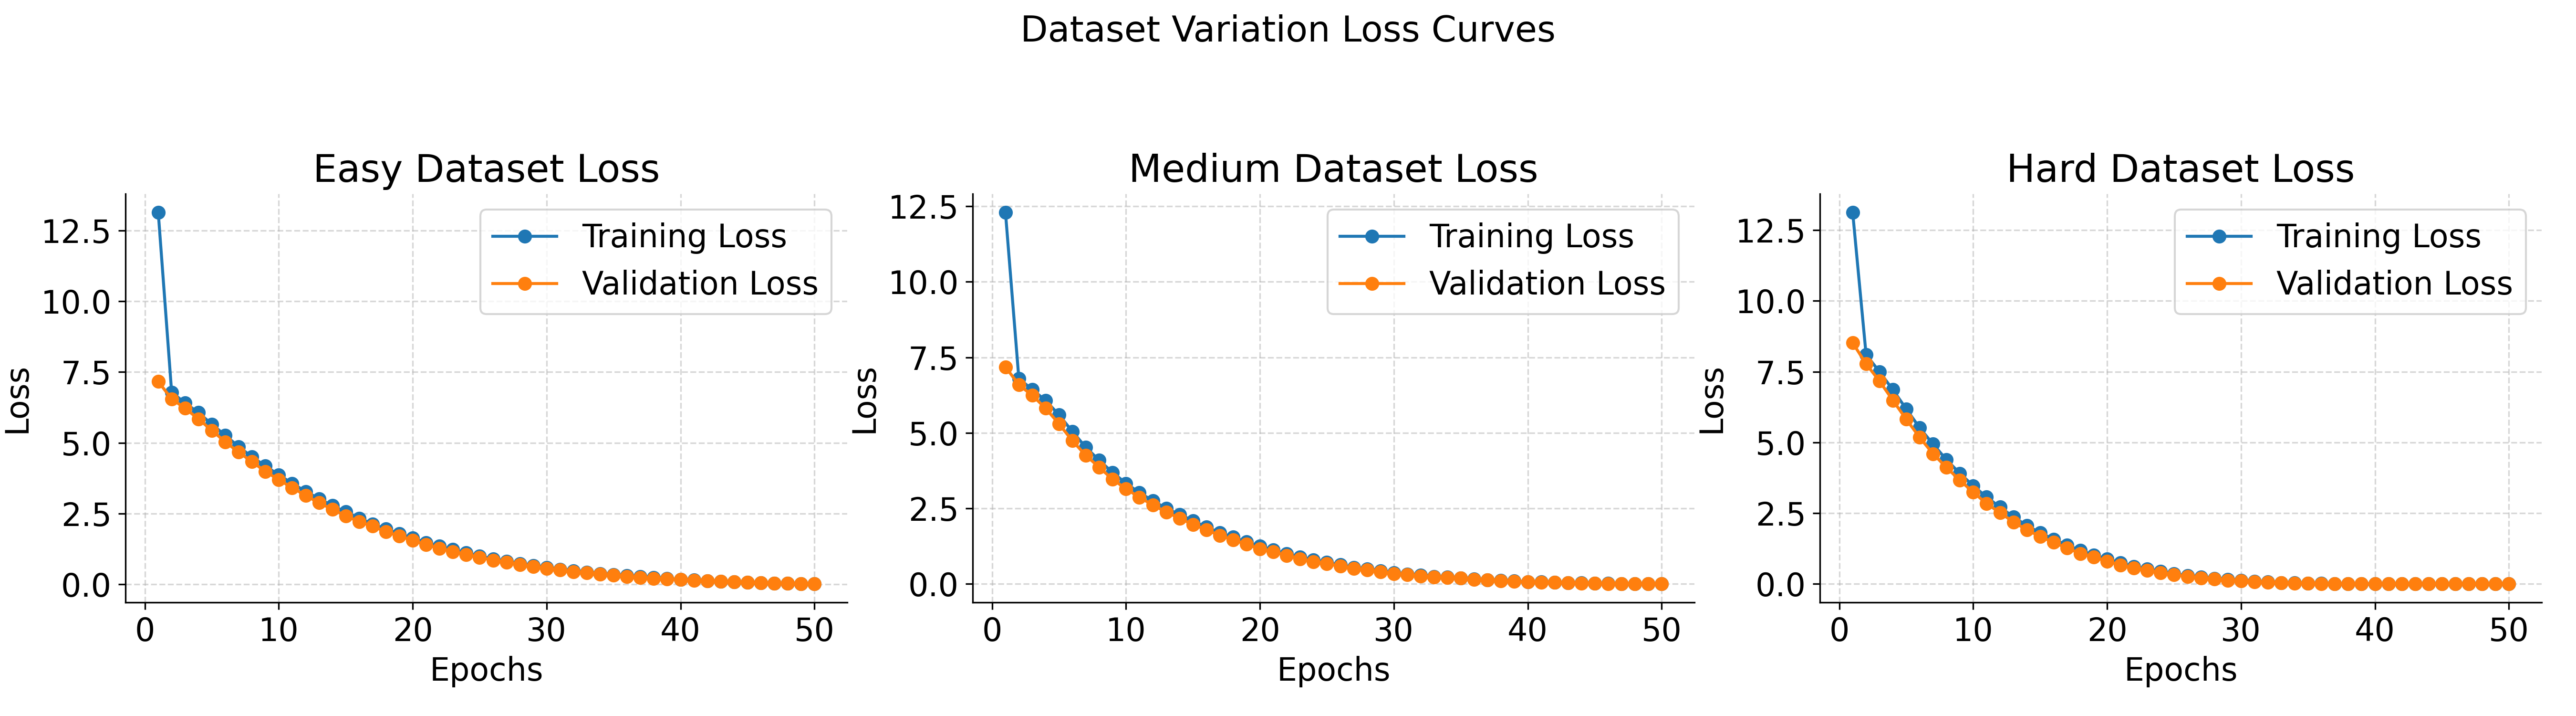
\includegraphics[width=0.95\textwidth]{img/3_dataset_variation_loss_curves.png}
    \label{fig:3_dataset_variation_loss_curves}
}
\subfigure[Regularization Loss Curves]{
    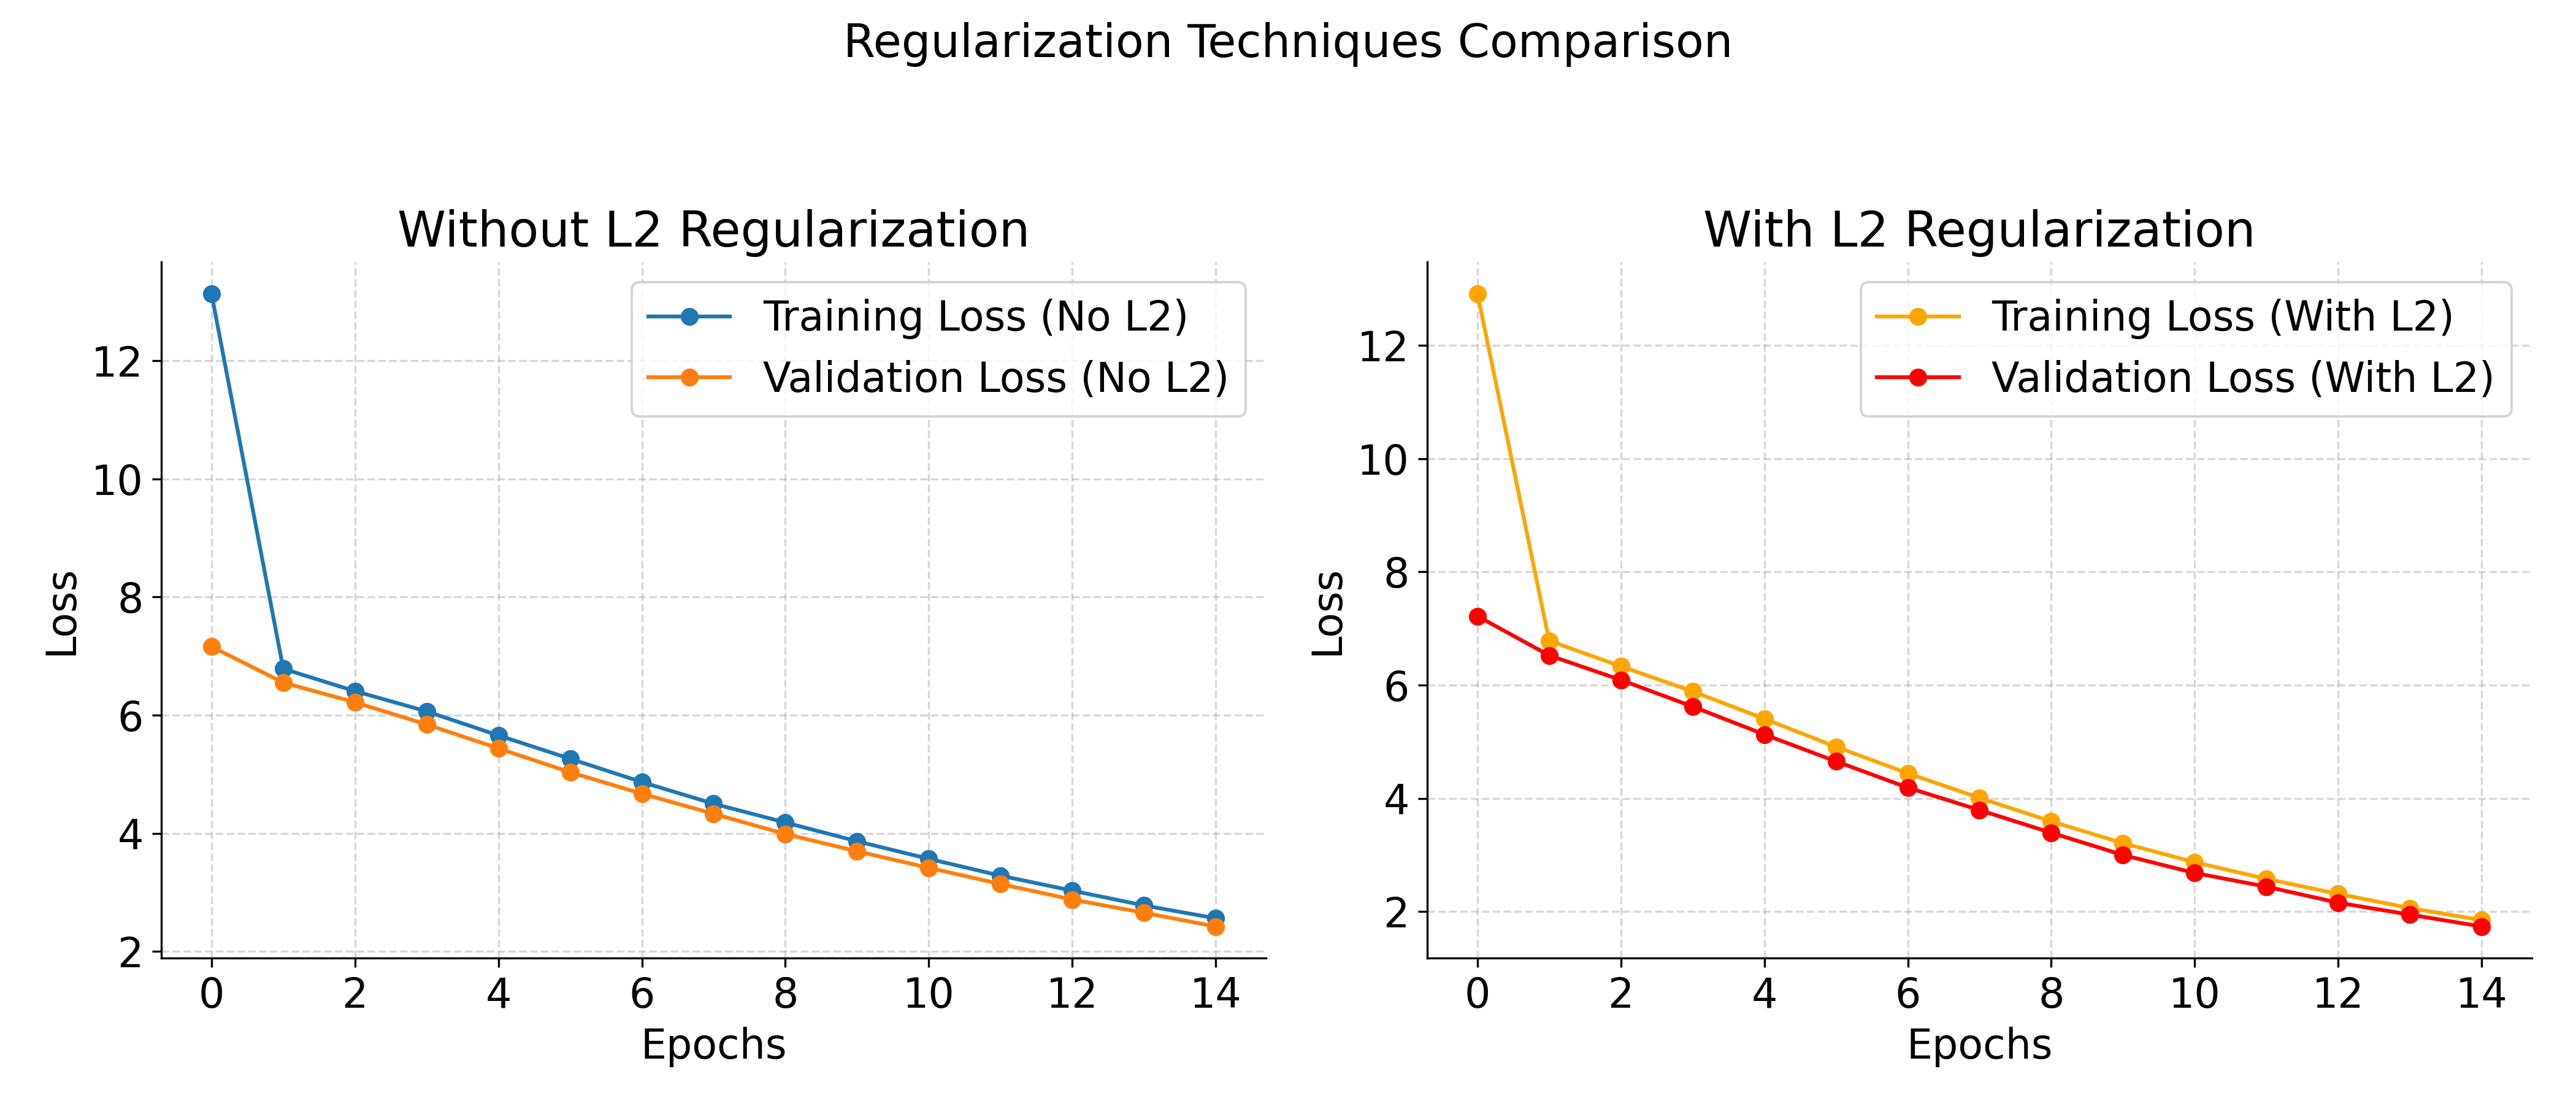
\includegraphics[width=0.75\textwidth]{img/4_regularization_loss_curves.png}
    \label{fig:4_regularization_loss_curves}
}
\caption{Performance evaluation across various experiments.}
\end{figure}

\section{Related Work}
The challenges associated with MDMs include computational inefficiencies and suboptimal decoding strategies. Prior works have demonstrated the success of ARMs in structured tasks \citep{zheng2024maskeddm, kim2025trainft}, but lack a comprehensive analysis of adaptive inference techniques. Recent advancements in adaptive inference-time computation have shown promise in enhancing generative models \citep{manvi2024adaptiveic}. Our study builds on these foundations, employing insights from adaptive sampling frameworks to optimize token selection and improve decoding efficiency in MDMs \citep{lee2023textconditionedsf, gwak2025rewardweightedse}.


\begin{figure}[h!]
\centering
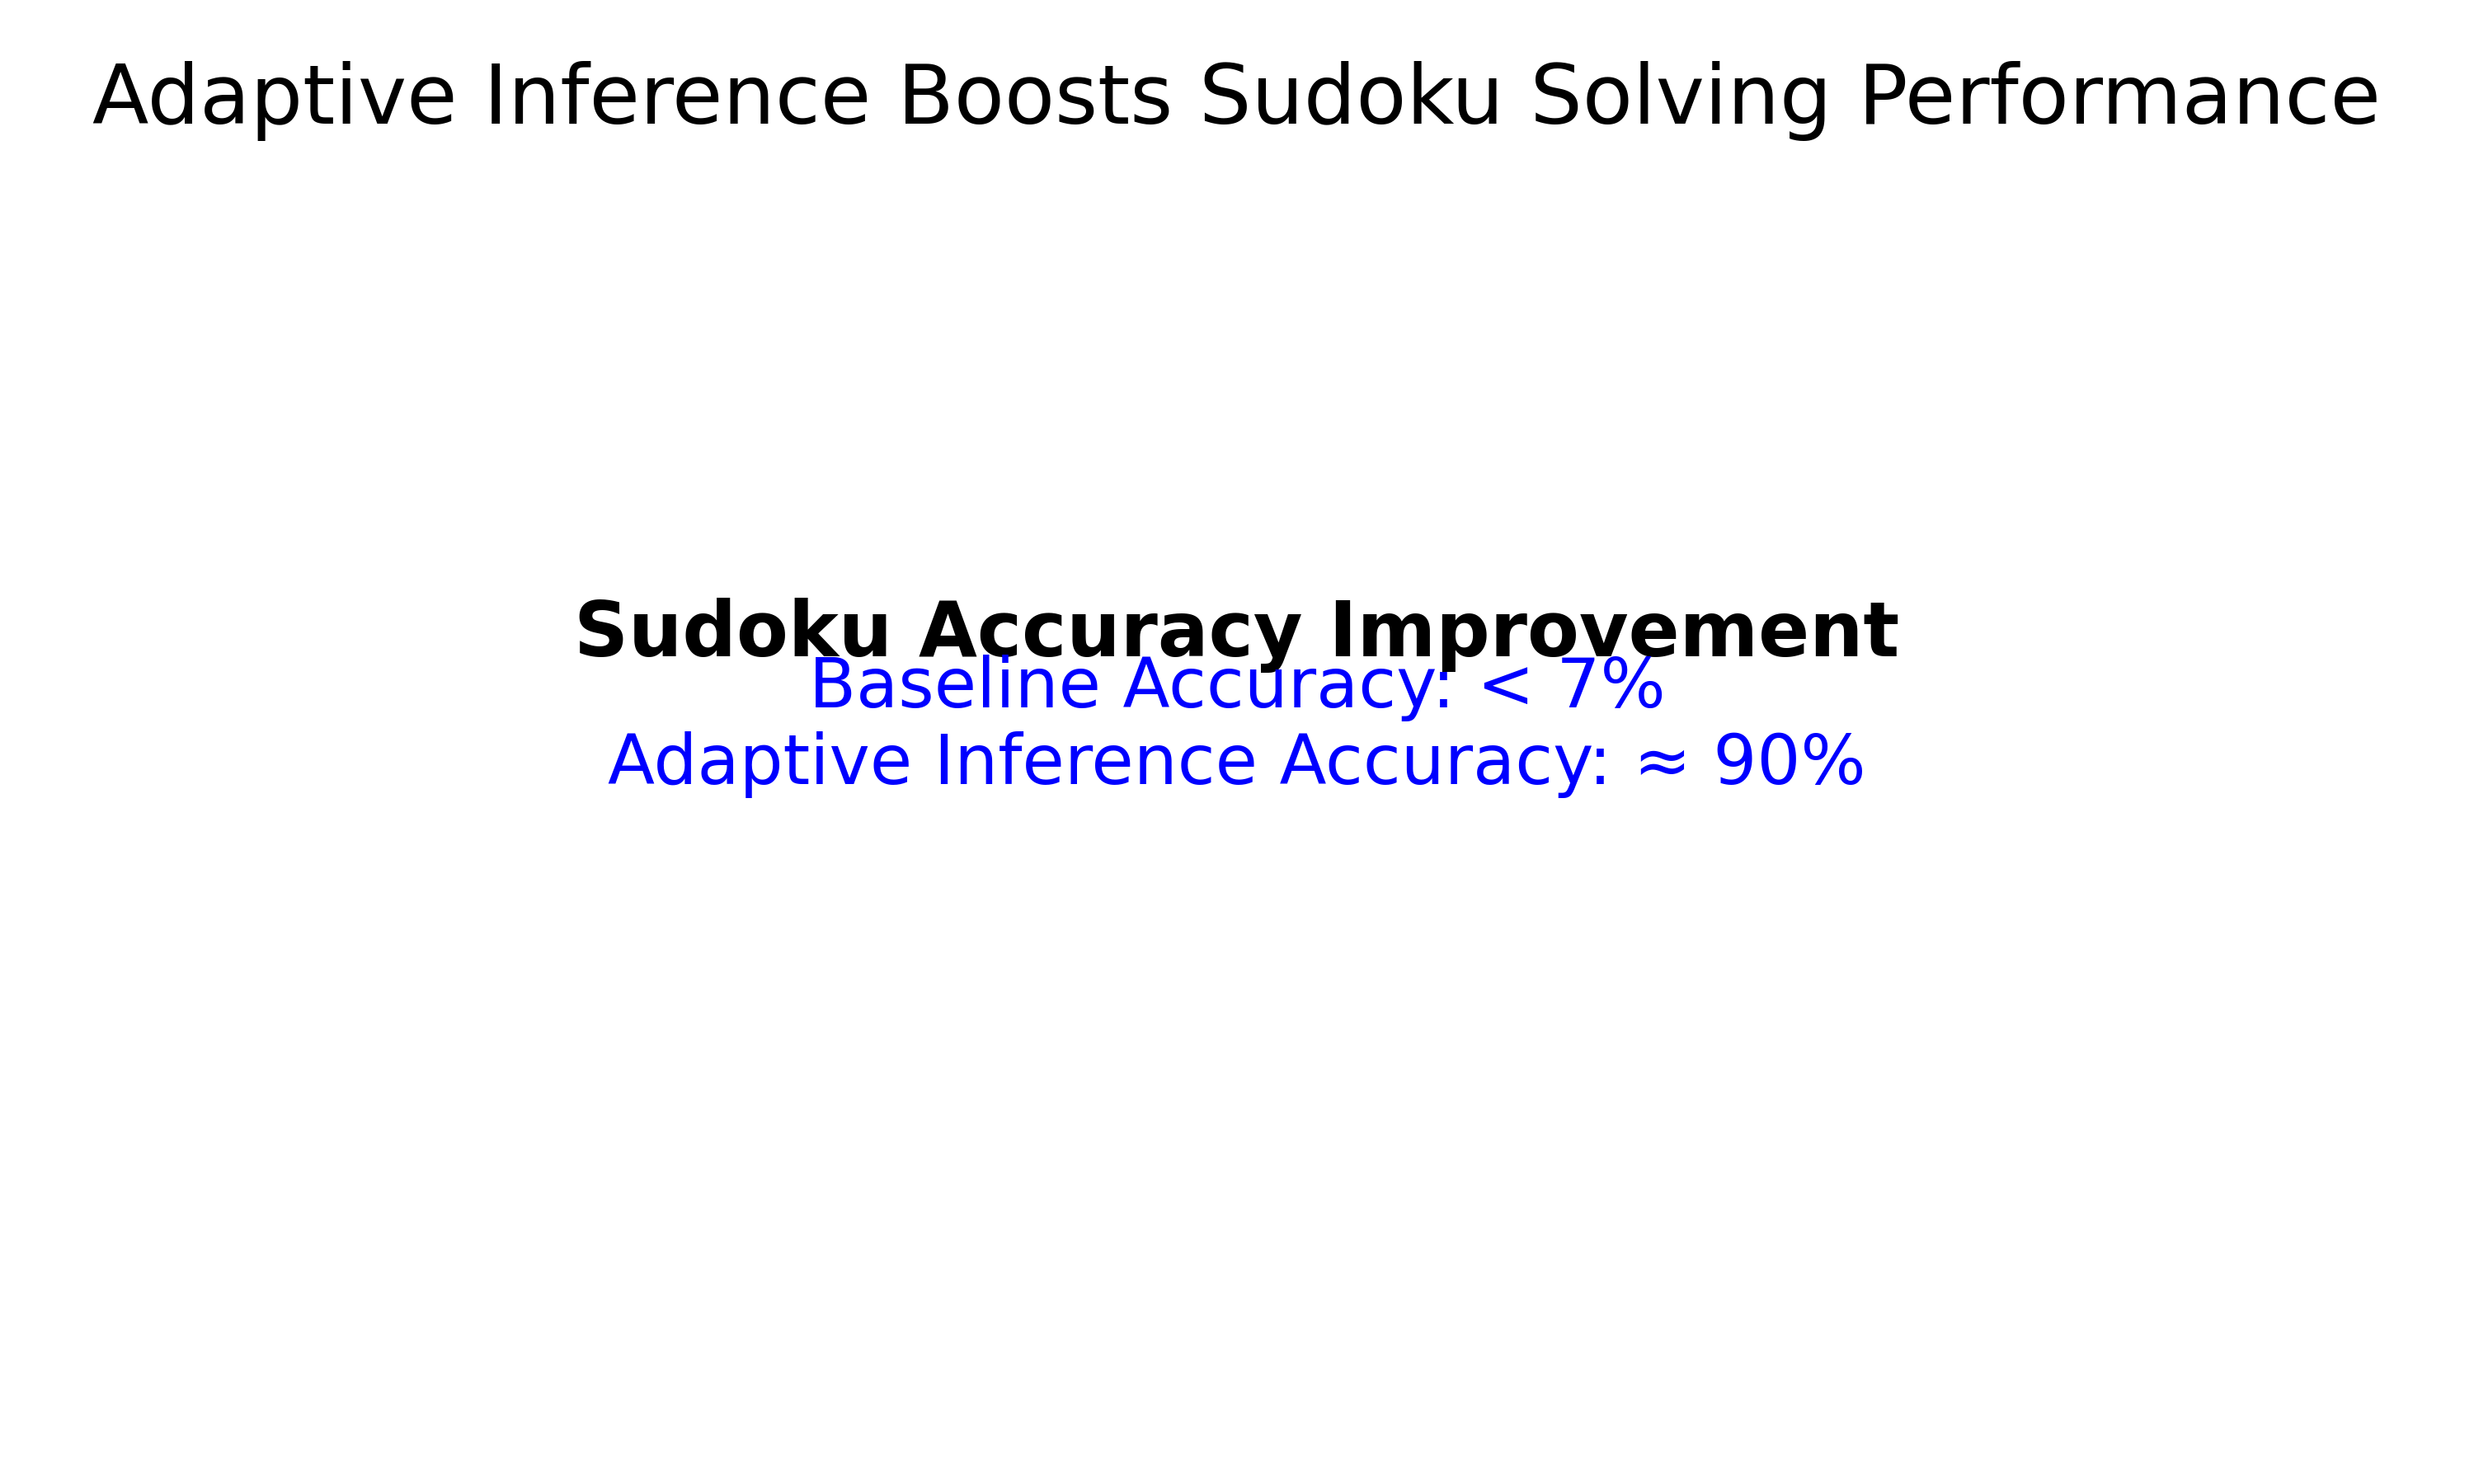
\includegraphics[width=0.6\textwidth]{img/11_adaptive_inference_accuracy.png}
\caption{Adaptive Inference Boosts Sudoku Solving Performance. Baseline accuracy: $<$ 7\%, Adaptive inference accuracy: $≈$ 90\%.}
\label{fig:adaptive_inference_accuracy}
\end{figure}



\section{Method}
We introduce adaptive inference strategies to dynamically adjust token ordering during the decoding phase of MDMs. This method leverages contextual information to prioritize token predictions, enabling the model to avoid computationally intensive subproblems. By evaluating the performance of different token sequences based on prior context, our approach enhances the model's ability to generate coherent outputs efficiently. This strategy is grounded in the theoretical framework of energy minimization \citep{chen2025maskeddm}, where optimal token arrangements can be derived to minimize generation errors.




\section{Experimental Setup}
To evaluate our adaptive inference strategies, we focused on Sudoku puzzles as a benchmark task. We established a baseline by comparing the performance of a standard MDM and an ARM under traditional decoding methods. Our experiments involved implementing an adaptive decoding strategy that selects token orders based on contextual cues. We assessed the resulting performance on Sudoku and other logic puzzles, measuring solving accuracy and completion time against baseline models.

\section{Experiments}
Our experiments revealed notable improvements in Sudoku solving accuracy, as illustrated in \cref{fig:adaptive_inference_accuracy}. The adaptive inference strategy achieved approximately 90\% accuracy, a significant leap from the baseline accuracy of less than 7\%. We also present loss curves and performance comparisons across various configurations.


Further analysis of the training and validation losses across different tasks is shown in \cref{fig:1_baseline_loss_curves,fig:2_activation_functions_loss,fig:3_dataset_variation_loss_curves,fig:4_regularization_loss_curves}. These results indicate that our adaptive strategies not only enhance accuracy but also improve convergence rates across a variety of configurations and datasets.



\section{Conclusion}
In conclusion, our research demonstrates the potential of adaptive inference strategies to significantly enhance the performance of masked diffusion models in solving complex generative tasks. By dynamically adjusting token ordering, we allow MDMs to sidestep computationally intensive subproblems, resulting in remarkable improvements in accuracy. Future work will explore the generalizability of these strategies across diverse tasks and their integration into real-time applications.


\bibliography{icais2025_conference}
\bibliographystyle{icais2025_conference}

% \appendix
% \section{Appendix}


\end{document}
